\documentclass[main.tex]{subfiles}
\begin{document}

\section{Digitized Waveform Neutron Tagging}

\subsection{Energy Calibrated NE213 QDC Spectrum}
By splitting the signals from the detectors it was possible to record data from the digital setup in parallel with the analog setup. A total of 2.3 million pulses were seen in the NE213 detector by the digitizer during one hour of measurements. The pulses were integrated digitally over the same gate lengths used in the analog setup, namely 60 and 500 ns starting 25 ns before the CFD trigger. A major difference relative to the analog setup lies in the baseline determination. For the analog setup we needed the pedestal in the energy calibration in order to account for and subtract any baseline offset. It acts as a global baseline subtraction. This is not necessary in the digital setup since the baseline is subtracted on an event by event basis during the initial data processing. 

The energy calibration was carried out using the 2.23 and 4.44 compton edges produced by the PuBe source as well as a $^{60}Co$ source were used. The energy calibration was performed with the Knox method as was the case for the analog setup. The 2.23 and 4.44 $MeV_{ee}$ compton edges are marked in green and red respectively in the top plot in fig \ref{fig:D_QDC}. The $^{60}Co$ source has compton edges at 1.17 and 1.33 $MeV_{ee}$, but only one edge is visible. It is assumed that this is the 1.33 $MeV_{ee}$ edge and that the 1.17 $MeV_{ee}$ edge lies beneath it. 

Unfortunately the baseline shift on the NE213 channel offset was set too high, at 40\%, reducing the range available to negative pulses to only 0.6 V. This particularly affects the 4.4 $MeV_{ee}$. It also affects cosmic rays, but these would still have been beyond the dynamic range if the full 1 V had been available.

As the middle panel of fig \ref{fig:D_QDC} shows the points still follow a linear trend in spite of some of them being out of range. The fit parameters are used to produce the calibrated energy spectrum shown below. 

\textbf{will be updated:}The peak near $12 MeV_{ee}$ is most likely cosmic muons. Travelling straight through the detector with desity. CONFIRM... $\rho=0.874g/cm^3$, $dE*cm^2/g=2MeV/g*cm^2$, $\rightarrow dE/dx= 1.748MeV/cm$, $dx=15$, $\rightarrow 26.22 MeV$. Then we would expect cosmic muons to leave this energy, but since their amplitude is out of range in the body of the pulse they will land in a lower QDC channel.

\begin{figure}[ht]
    \centering
        \includegraphics{DigitalResults/Ecall.pdf}
        \caption{The 1.17 + 1.25 MeV edge of the $^60$ source and the 2.23 and 4.44 MeV Compton edges of the PuBe source have here been used to perform an energy calibration. Due to the event by event based baseline determination it is assumed that bin 0 corresponds to 0 $MeV_{ee}$}
    \label{fig:D_QDC}
\end{figure}


\clearpage
\subsection{Pulse shape discrimination}
\subsubsection{Charge comparisson method}
Just like with the analog setup the charge integrals were used to perform pulse shape discrimination. The resulting PSD heatmap is shown fig \ref{fig:psd_d}. Since a lower amplitude threshold was applied to the digital setup we find a lot of low energy gammas in the gamma bad. The 2.23 $MeV_{ee}$ and 4.44 $MeV_{ee}$ compton edges are also clearly distinguishable. 

As with the analog setup longgate and shortgate offsets can be used to linearize the seperation between the bands. Here each shortgate sample point has been offset by 5 mV while each longgate sample has been offset by 0.26 mV. At lower energies the bands intersect, but above 1.5 MeV they are clearly separated.

\begin{figure}[ht]
    \centering
        \includegraphics{DigitalResults/psd.pdf}
        \caption{Pulse shape discrimination spectrum produced with the charge comparisson method.}
        \label{fig:psd_d}
\end{figure}

\subsubsection{Convolutional neural network based discrimination}
The convolutional neural network described in \ref{sec:cnn} was applied to the digitized waveforms. Since the activation function of the output node is the logistic function the value is bounded between zero and 1. The resulting pulse shape discrimination spectrum is shown in fig \ref{fig:cnn_E} as a function of deposited energy. Like for the charge comparisson method the upper distribution is neutrons and the lower distribution consists of gamma. The bands a much better separated than by the charge comparisson method although the still is some slight overlap at low energies. Again the 2.23 and 4.44 $MeV_{ee}$ compton edges are clearly visible in the gamma band. It is interesting that the 4.44 $MeV_{ee}$ edge is much less spread out than the 2.23 $MeV_{ee}$ edge. This might be because the neotron pulses rarely go out of range, so the network has learned to associate pulses that go out of range (and so have a flat peak) with gammas.


\begin{figure}[ht]
    \centering
        \includegraphics{DigitalResults/CNNpsd.pdf}
        \caption{Pulse shape discrimination spectrum produced with a convolutional neural network.}
    \label{fig:cnn_E} 
\end{figure}

\clearpage
\subsection{Time of flight spectrum}
The time of flight spectrum acquired in the 1 hour of data taking is shown in fig \ref{fig:tof_d}. The gamma and netron peaks are indicated with arrows. The gamma peak is not entirely narrow as one might expect seeing as they all travel at the speed of light. As for the analog setup part of the reason is that each photon may have a longer or shorter flightpath depending on its point of production in the source and the point at which it interacts in the detector. Furthermore, the time resolution is limited by is limited by the digitization process. The CFD algorithm looks for where the pulse crosses 30\% of maximum amplitude, but the determination of the maximum amplitude is limited by the resolution and sampling rate of the digitizer.

The flight time in the neutron peak, marked with dotted red lines, has been used to generate the energy spectrum shown in the upper right insert of fig \ref{fig:tof_d}. The spectrum goes to lower energies than what we see for the analog setup in fig \ref{fig:tof_a}, this may be because the digital setup has a lower amplitude threshold than the analog setup, allowing slower neutrons to be recorded.
\begin{figure}[ht]
    \centering
        \includegraphics{DigitalResults/tof.pdf}
        \caption{The time of flight spectrum of the PuBe source produced by the digital setup.}
    \label{fig:tof_d} 
\end{figure}

In order to test the two pulse shape discrimination algorithms we can plot their pulse shape parameters against time of flight. This is shown in figure \ref{fig:tof_cc_tof_cnn}. In fig \ref{fig:tof_digi_cc} we see the narrow gamma distribution and the wider neutron distribution. It is apparent that the two distributons overlap somewhat. The neutron and gamma background forms to bands.  In fig \ref{fig:tof_digi_cc} the distribution are better separated, but it still appears that gammas and neutrons overlap slightly near prediction value 0.5. The distribution of random coincidence events clearly separate into a gamma band at CNN prediction value 0-0.3, and a neutron band at prediction value 0.7-1.


\begin{figure}
    \centering
    \begin{subfigure}[ht]{\textwidth}
        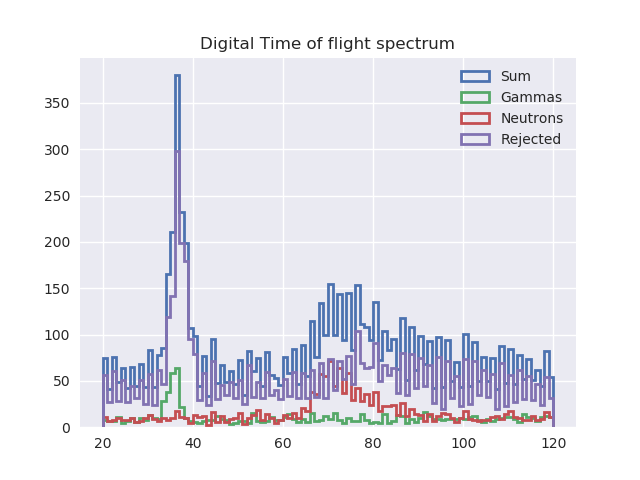
\includegraphics{DigitalResults/tof_psd.pdf}
        \caption{}
        \label{fig:tof_digi_cc}
    \end{subfigure}
	\begin{subfigure}[ht]{\textwidth}
        \includegraphics{DigitalResults/CNNtof_psd.pdf}
        \caption{}
        \label{fig:tof_digi_cnn}
    \end{subfigure}
    \caption{heatmaps of of pulseshape discrimination parameters as functions of time of flight plotted with logarithmic z-axis.}
    \label{fig:tof_cc_tof_cnn}
\end{figure}

If we expand the time of flight spectrum along the particle energy axis we get the heatmap shown in fig \ref{fig:tof_E_d}. This spectrum can help us understand why the gamma spectrum is not entirely narrow. It seems that low energy gammas are a bit more spread out regarding time of flight. This could mean that the CFD algorithm has a harder time timestamping low charge pulses.
% or perhaps that low energy gammas travel a longer distance into the detector before they interact.
If we now look at the relation between deposited energy and neutron kinetic energy we see the same trend as for the analog setup. A neutron may deposit all or part of its energy, so for a given deposited energy we can only conclude the minimum amount of energy the neutron must have had.


\begin{figure}[ht]
    \centering
        \includegraphics{DigitalResults/tof_E.pdf}
        \caption{Time of flight plotted against energy deposition.}
    \label{fig:tof_E_d} 
\end{figure}

\begin{figure}[ht]
    \centering
        \includegraphics{DigitalResults/tof_Edep_Eneutron.pdf}
        \caption{Neutron energy as a function of deposited energy in the NE213 detector.}
    \label{fig:tof_Edep_Eneutron_d} 
\end{figure}




\end{document}